\section{Forging Process Simulator}
% 本研究构建了一个基于深度算子网络（DeepONet）的代理模型，用于在给定锻压参数下同步预测位移场、应力场和损伤场的时空演化。该模型学习由控制量与扰动决定的物理场预测算子，实现多场耦合与全时域一体化建模。

% 锻造过程被表述为依赖于初始温度场和工艺参数的演化问题。模型输入包括工艺参数（分支网络处理的速度曲线参数 $\theta = \{v_0, v_1, t_0, t_1\}）$和时空信息（主干网络处理的空间坐标$ (x, y, z)、SDF、时间步step 和初始温度 Temp）$。基于算子学习框架，模型具备全时域预测能力，一次前向传播即可直接输出对应时间步 step 的物理状态，结构如图\ref{fig:model}所示。
% \begin{figure}[htbp]
% \centerline{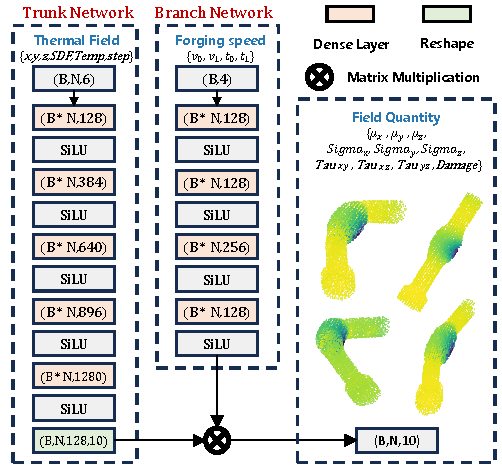
\includegraphics[width=\linewidth]{model.pdf}}
% \caption{Field value prediction model.}
% \label{fig:model}
% \end{figure}

% 模型目标是学习一个算子G，建立如下映射关系：
% \begin{equation}
% G:(\theta)(x,y,z,SDF,step,Temp)\to(\mu,\sigma,d)
% \end{equation}
% 其中 $\mu$、$\sigma$ 和 $d$ 分别表示位移场、应力场和损伤场。为捕捉变形与应力的强耦合关系，模型采用共享输出层设计：分支网络提取参数特征 $B = [b_1, b_2, \dots, b_p]$，主干网络提取时空特征$ T = [t_1, t_2, \dots, t_q]$，二者融合后通过共享权重输出联合物理场：
% % \begin{equation}
% %     \mathbf{y}(x,y,z,step) \approx W \cdot (B \otimes T) + b_0
% % \end{equation}

% % \begin{equation}
% % \begin {split}
% %  \mathbf{y}(x,y,z, step) &= [u(x,y,z, step), \\
% %      &\sigma(x,y,z, step), d(x,y,z,step)]
% % \end{split}
% % \end{equation}

% \begin{equation}
% \begin{split}
% \mathbf{y}(x,y,z,step) &\approx W \cdot (B \otimes T) + b_0 \\
% \mathbf{y}(x,y,z, step) &= [u(x,y,z, step), \\
%      &\sigma(x,y,z, step), d(x,y,z,step)]
% \end{split}
% \end{equation}

% 其中$W$是共享输出层的权重矩阵，$b_0$是偏置向量。该设计通过统一映射机制同步输出多物理场，强化了耦合关系学习，保障了物理一致性。

% 训练过程通过最小化预测与真实数据之间的均方误差进行：
% \begin{equation}
% \mathcal{L} = \frac{1}{N} \sum_{i=1}^{N}
% \left\|
% \left[ \mathbf{y}^{(i)} \right] -
% \left[ \mathbf{y}_\text{true}^{(i)} \right]
% \right\|^2
% \end{equation}
This work develops a DeepONet-based surrogate model to predict the
coupled spatiotemporal evolution of displacement, stress, and damage
fields during forging. The model learns the underlying physics operator
for full-time-domain prediction.

The process is modeled as an evolution problem dependent on the initial
temperature field and speed parameters
$\theta = \{v_0, v_1, t_0, t_1\}$. Inputs are $\theta$ (branch net) and
spatiotemporal coordinates $(x, y, z, SDF, step, Temp)$ (trunk net). A
single forward pass outputs the state at any given time step
(Fig. \ref{fig:model}).

The model learns the operator $G$:
\begin{equation}
G: (\theta)(x, y, z, SDF, step, Temp) \rightarrow (u, \sigma, d)
\end{equation}
where $u$, $\sigma$, $d$ are displacement, stress, and damage. A shared
output layer captures field couplings. Branch and trunk outputs $B$ and
$T$ are fused as:
\begin{equation}
\mathbf{y} = [u, \sigma, d] = W \cdot (B \otimes T) + b_0
\end{equation}
This unified mapping ensures physical consistency. Training minimizes
the mean squared error:
\begin{equation}
\mathcal{L} = \frac{1}{N} \sum_{i=1}^{N} \left\| \mathbf{y}^{(i)} - \mathbf{y}_{\text{true}}^{(i)} \right\|^2
\end{equation}
